\chapter{\textit{Novelpy}: A \textit{Python} Package to Measure Novelty and Disruptiveness of  Bibliometric and Patent Data}
\markboth{CHAPTER 3. \textit{NOVELPY}}{CHAPTER 3. \textit{NOVELPY}}

\begin{chapabstract}{\small Pierre \textsc{Pelletier}} % if co-authored, else juste start by \begin{chapabstract}{} as in chapter 2
     \small \textit{Novelpy} (v1.2) is an open-source \textit{Python} package designed to compute bibliometric indicators. The package aims to provide a tool for the scientometrics community that centralizes various measures of novelty and disruptiveness, enables their comparison, and fosters reproducibility. This paper offers a comprehensive review of the different indicators available in \textit{Novelpy} by formally describing these measures (both mathematically and graphically) and presenting their advantages and limitations. We then compare the different measures on a random sample of 1.5M articles drawn from the Pubmed Knowledge Graph to demonstrate the module's capabilities. We encourage anyone interested to participate in the development of future versions.
\end{chapabstract}


\section{Introduction}
\label{sec:introduction}

Identifying and tracking relevant pieces of knowledge remains a core issue in the Science of Science research. A better understanding of knowledge flow dynamics, mechanisms behind the emergence of new ideas, and identification of novel or impactful documents are crucial for fostering effective science, which will, in turn, help address future societal challenges \citep{fortunato2018science, foster2021surprise, ocde}.
This article proposes integrating various bibliometric indicators within a \textit{Python} package. It assembles within a single module novelty or, more broadly, creativity measurements through combinatorial novelty indicators \citep{uzzi2013atypical,foster2015tradition,lee2015creativity,wang2017bias,shibayama2021measuring}, as well as several impact measures, including disruptiveness metrics \citep{wu2019large,wu2019solo,wu_wu_2019,bu2019multi,bornmann1911disruption}.

This module is intended for researchers in the emerging and multidisciplinary field of Science of Science. There is an increasing tendency to create new scientometric indicators, but there are fewer initiatives to design reproducible experiments. For novelty indicators, there is minimal reference to prior approaches when creating a new indicator; thus, the flexibility in the choice of measures raises the temptation to choose the measure that produces the intended outcome \citep{foster2021surprise}. Only a few studies attempt to establish a conceptual background of creativity and the formalization of the indicators \citep{foster2021surprise}. This article provides a mathematical and graphical description of these indicators. To the best of our knowledge, it is the first tool that enables the computation of these metrics.

Two macro types of analysis can describe Scientometrics: performance analysis and Science Mapping Analysis (SMA) \citep{moral2020software}. Performance analysis aims to assess the activities of scientific actors and their impact. Its purpose is to assign a value to the productivity and pervasiveness of research conducted by a unit (article, author, institution). SMA "is mostly directed at monitoring a scientific field to determine its (cognitive) structure, its evolution, and main actors within" \citep{noyons1999integrating}. It captures a snapshot of a part of the scientific system at a given moment to analyze its structure. The present package allows performing analysis through disruptiveness measures; it also assesses the creative potential of papers using novelty indicators. Both metrics require science mapping analysis to be measured since they are generated through maps of the structure of science. Inputs, outputs, and impacts of these scientific activities are the three perspectives used in bibliometric analysis \citep{sugimoto2018measuring}\footnote{\justifying Input refers to human and financial resources and captures the different interactions of agents in the system at various levels (authors/institutional/country levels). Output results from the research process, the different entities that characterize a document. Finally, impact measures knowledge dissemination generated by an article through citations, attention by the general public, or re-utilization of a document's components.}. Entities involved in most combinatorial novelty indicators use only the output part of documents to compute their measures \citep{uzzi2013atypical, foster2015tradition, lee2015creativity, shibayama2021measuring}, except for \cite{wang2017bias}, which uses references from future articles to control for re-utilization. Disruptiveness indicators \citep{wu2019large, bu2019multi, bornmann2020disruptive} take the outputs and impacts of a given document to construct their metrics. They are based on both the references and citations of a given document. This module focuses on metrics using outputs (references/keywords) and impact features (citations/references and keywords from future articles).
 
While citation is an invaluable source of information, several limitations exist when using the sheer number of citations to evaluate impact. Inter-field (and even intra-field) comparisons can be challenging, as the sheer number of scientists and the way science is performed vary significantly depending on the research domain (methodology, solo author vs. team publication, citation habits). The gap in the number of citations is mainly due to the field's structure and does not necessarily represent the documents' quality. This phenomenon becomes an issue when raw numbers are used to measure the importance of research \citep{purkayastha2019comparison}. The same problem arises with self-citation, comparing national and international journals, or document languages \citep{van2001language}.

Network effects have been observed in citation dynamics. \cite{wallace2012small} showed that scholars tend to cite researchers with whom they have a deeper social connection. They also found that researchers are more likely to cite collaborators of collaborators, thereby creating a citation continuum. Articles with international collaborations are more cited due to network effects \citep{wagner2019international}. Other negative citation behaviors arise in \cite{bornmann2008citation}; scholars tend to cite papers to satisfy editors and reviewers, showing an apparent disconnection between citation and actual importance during the creation process. Field-specific issues can be addressed using normalization methods or different counting methods of citations (see \cite{waltman2016review} for a comprehensive review).
One family of normalized indicators is disruptiveness \citep{wu2019large,wu2019solo,wu_wu_2019,bu2019multi,bornmann1911disruption}. These measures analyze how a focal article acts as a bottleneck between future papers and the references of the focal papers. They capture whether a document consolidates a domain (i.e., future papers rely on the same pieces of knowledge as the focal paper) or constitutes a starting point for documents from various areas (i.e., future papers only use information from the document).

Scientific advancement is the result of individuals' creativity, where \textit{creativity} is defined as "\textit{held to involve the production of high-quality, original, and elegant solutions to complex, novel, ill-defined, or poorly structured problems}" \citep{hemlin2013leadership}.
Scholars have proposed measurements to complement these impact indicators with creativity indicators, usually called ``atypicality'', originality'', or ``novelty'' indicators. The need for quantifying novelty comes from its position as an essential component of the structure of the scientific and economic system. Novelty is at the origin of peer recognition, which acts as a "reward system" for individuals. The "priority rule" grants recognition to the first person making the discovery \citep{merton1957priorities, carayol2019}. Novelty is also at the core of the theory developed in evolutionary economics, in which technological progress and creativity influence the cyclical nature of the economy \citep{schumpeter1939business,nelson1985evolutionary,amendola2014novelty}. Scientific progress remains elusive, and novelty indicators are intended to approach creativity, as making relevant novel combinations is perceived as innovative \citep{burt2004structural,rodriguez2016research,bornmann2019do}. The earliest novelty indicators focused mainly on past information (i.e., using an entity created the same year) or the distance between articles from a given year, based on their references' overlapping \citep{dahlin2005invention}.

More recently, scholars have integrated the conceptual framework of knowledge recombination (a combination of pre-existing ideas that leads to invention) into novelty indicators. This concept was already developed by \cite{poincare1910mathematical}. Although he refers to the specific case of science, it can be extended to any type of non-scientific creative process where combinations can be both material and conceptual \citep{winter1982evolutionary}. \cite{weitzman1998recombinant} discussed how knowledge could be generated through a combinatorial process of past ideas and how this can generate economic growth as long as potential new ideas are exploitable. At the same time, an invention does not necessarily arise from combining two components together for the first time. Indeed, it can also arise from creating a new relationship between two already linked components \citep{schumpeter1939business, henderson1990architectural}. This deepens the idea brought by \cite{jacob1977evolution} that scientific advancement emerges from looking at something from a new angle rather than incorporating a new instrument. Scientists have proposed a more probability-based approach to capture this combinatorial process. Instead of focusing solely on the degree of novelty of a combination, they look at how unlikely this combination is to happen. The more distant the items in the combination, the more complex and unlikely it is to make this combination. Therefore, the combination is more novel. To solve mathematical problems, Poincaré used the knowledge he found in another field \citep{poincare1910mathematical}. The more distant the fields were, the more insight he gained. However, novel documents exhibit higher variance in citation performance. Academics adopting an exploration strategy face a higher risk of failure \citep{fleming2001recombinant,foster2015tradition,wang2017bias, ocde}. Indeed, scientific documents that have a fair mix of novel and conventional ideas are more likely to be ``sleeping beauties'' than other documents (see \cite{ke2015defining} and \cite{wang2017bias}). The idea of \cite{march1991exploration} that organizations which explore and consolidate existing processes/technologies are more likely to survive can also be applied in the scientific realm\footnote{\justifying Here, survival can be expressed as a high citation count.}. Novelty indicators can be applied to different entities (patents, papers, webpages, etc.) using various units of knowledge (references, keywords, MeSH terms, text, and others).

Most of the packages available in \textit{R} and \textit{Python} deal with performance or SMA. \cite{moral2020software} carried out a detailed and up-to-date review of the different tools and libraries that help researchers in their daily work. Although much work has been done to study citation, co-authorship, or any coupling, novelty and disruptiveness indicators are still unavailable, and researchers have to code these metrics themselves. Concerning the reproducibility of novelty studies, only \cite{shibayama2021measuring} shared their code on Github to calculate their new novelty indicator, but this is still an isolated event. This tool, therefore, ensures that indicators of novelty and disruption used in future studies will be replicable.

The rationale for incorporating novelty and disruptiveness indicators in a single package comes from the fact that they both capture different aspects of the documents: the former aims at quantifying the risky profile of research, looking at the balance between exploitation and exploration \citep{march1991exploration} of the knowledge space. At the same time, the latter analyzes how impactful an article is for science. The link between novelty and citation count has been of interest in previous research \citep{uzzi2013atypical,wang2017bias}, and more recently, \cite{lin2021new} studied the relationship between novelty and disruptiveness indicators. The different studies only look at specific novelty indicators, and a complete benchmark is still missing. This paper contributes to an ongoing effort to systematically benchmark and compare multiple indicators of impact and novelty by proposing an open-source tool to the community.

This article contributes to the Science of Science literature by providing an open-source \textit{Python} package, \textit{Novelpy}, to compute Novelty and Disruptiveness measurements. It unifies the existing indicators in a common framework using a formalization based on graph theory and provides some hands-on experience. We hope that \textit{Novelpy} will contribute to homogenizing our practice in the science of science and support researchers in their work. The package will be available in \textit{Python}, one of the most popular open-source programming languages (hence with the most prominent community support), and will be maintained long-term. The package currently works with a specific and documented data structure, but tools to easily use well-known data sources are under development. The package will be hosted on \textit{PyPI} and also on \textit{Github}, which allows the creation of bug reporting and/or proposition of development\footnote{\justifying Documentation is available here \url{https://novelpy.readthedocs.io/en/latest/usage.html}}. The rest of the paper is structured in the following way. In Section \ref{sec:indic} contains the formalization of the indicators that are implemented in \textit{Novelpy}. Section \ref{sec:resnovpy} demonstrates the package's capabilities on a random sample drawn from PubMed. We close the paper with a discussion on the remaining limitations of novelty indicators' usages and the purpose of the package.

\section{Supported indicators}
\label{sec:indic}

This section details the content of \textit{Novelpy}, describes the computation for each indicator, and the data required. The \textit{Novelpy} Python package provides a set of functions to perform quantitative analysis in scientometrics. The structure of the module is divided between novelty and disruptiveness indicators. Novelty indicators are also separated between indicators based on co-occurrence matrices and ones based on text embedding techniques, as represented in figure \ref{fig:mindmap}.

Practically, disruptiveness indicators are all calculated through the same function, while novelty indicators have a function for each measure. All functions are explained in the module's documentation (\url{https://novelpy.readthedocs.io/}).
    
    
    \begin{figure}[!h]
    \centering
        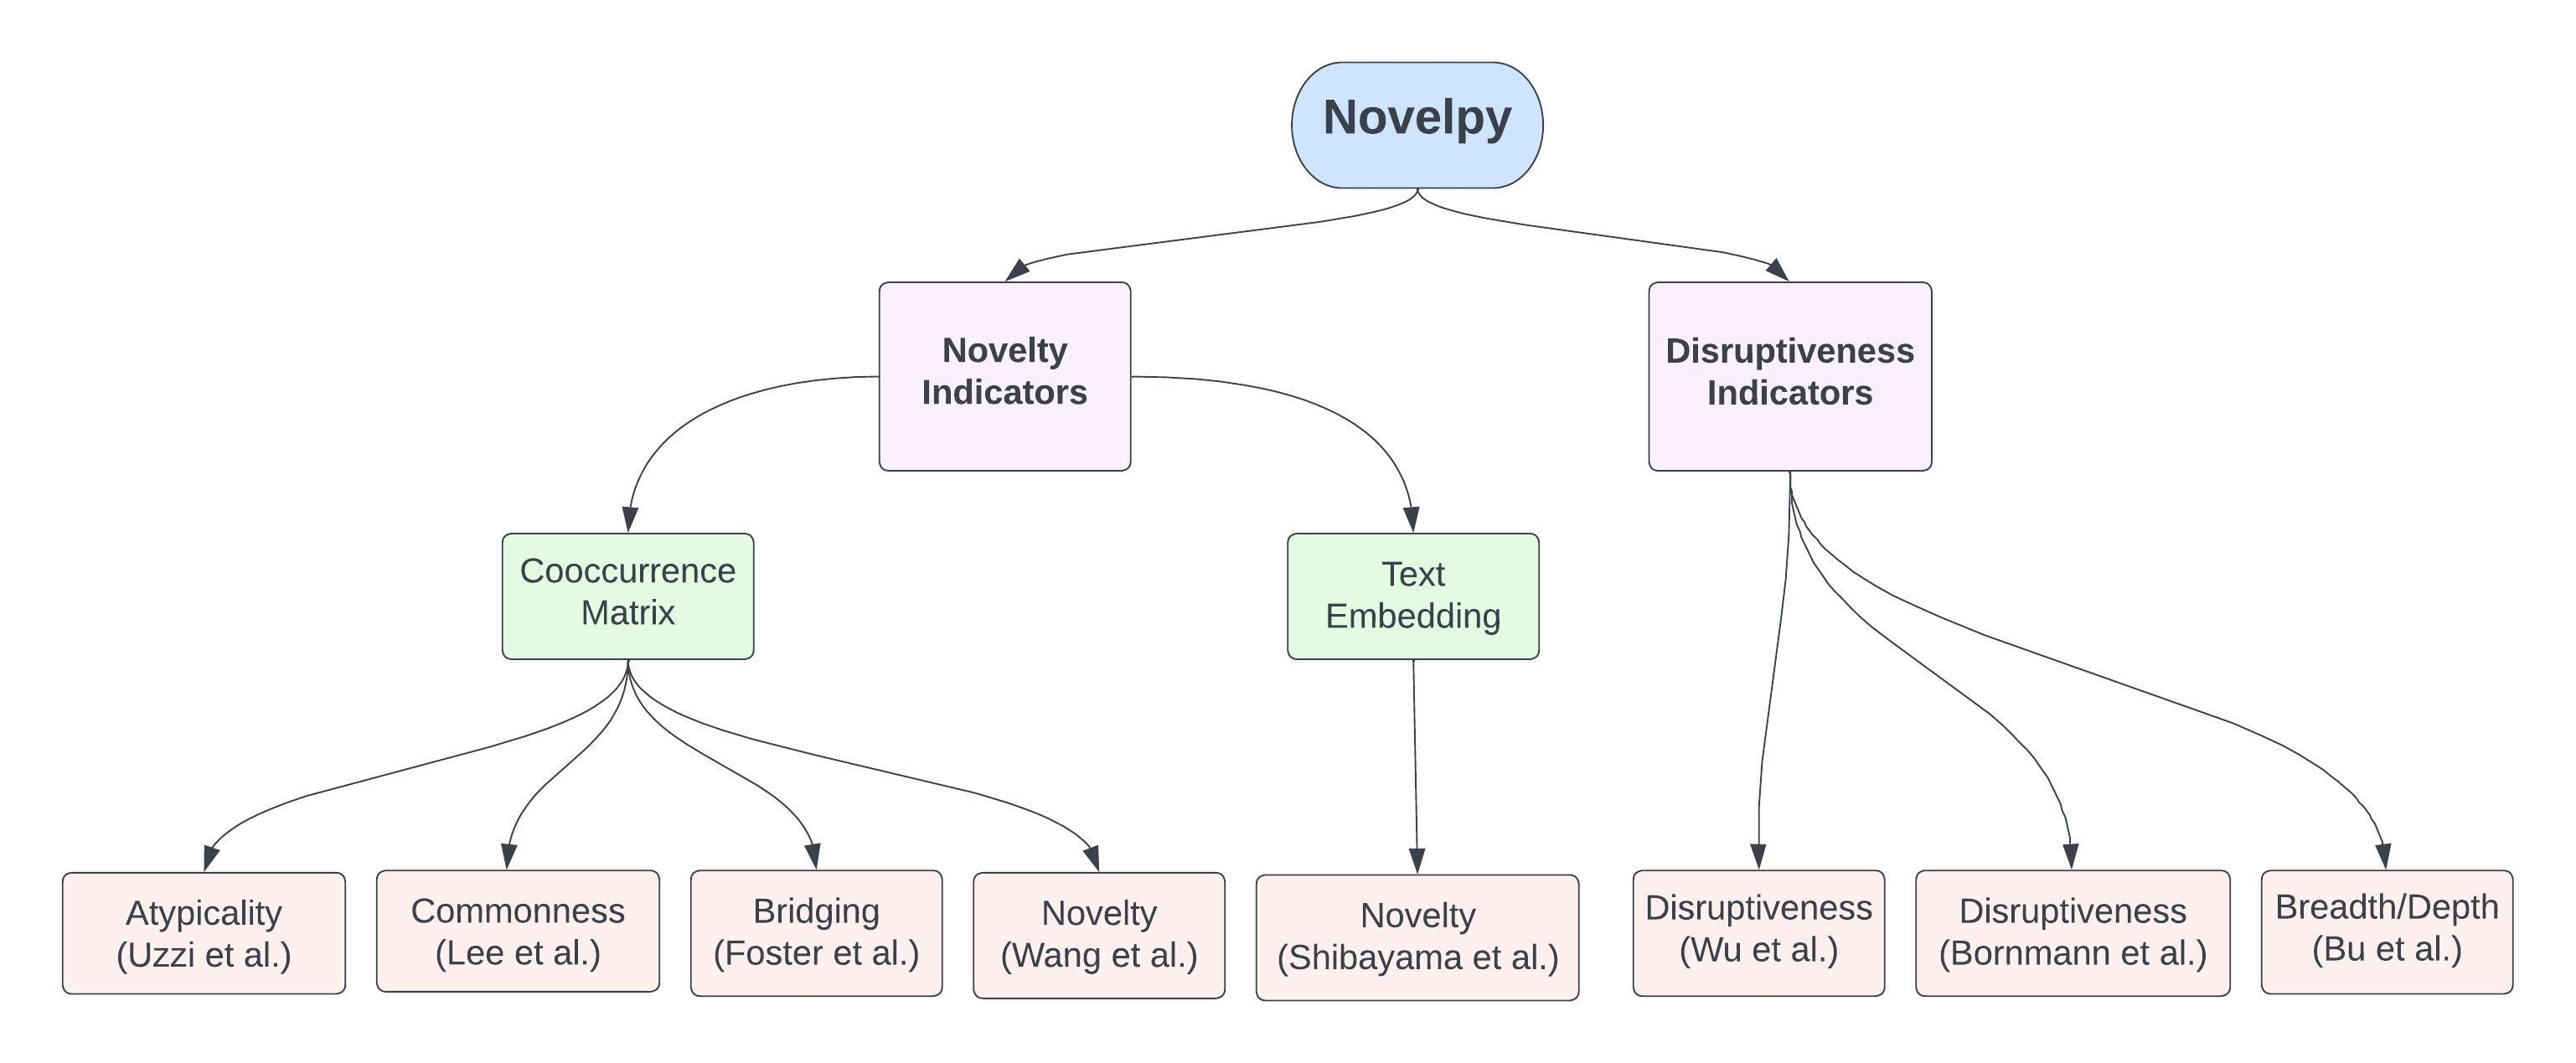
\includegraphics[scale= 0.585]{3_chapter3/figures/legende (2).jpeg}
          \caption[\textit{Novelpy}'s module structure]{\textit{Novelpy}'s module structure }
      \label{fig:mindmap}
    \end{figure}
    
Different data types can be employed depending on the indicator, as shown in \ref{tab:indicators}. All indicators working with a co-occurrence matrix can use references, journals, or keywords, and disruption indices rely on the citation network. \cite{shibayama2021measuring}'s indicators use the citation network and title or abstract to represent the article's semantics in a vector space. Various tools to preprocess bibliometric data are also included within the package to simplify the computation of proposed measures\footnote{\justifying see \url{https://novelpy.readthedocs.io/en/latest/utils.html}} (e.g., co-occurrence matrix construction, text embedding, citation and co-authorship network creation). Table \ref{tab:indicators} summarizes the indicators available in the module, their strengths and weaknesses, and the possible variables to compute them.
    
    
\begin{table}[!h]
\begin{adjustwidth}{-1cm}{}
    \scalebox{0.8}{
	\begin{threeparttable}
 
\renewcommand{\arraystretch}{1}
    \begin{tabular}{llll|c|c|c|c|}
    \toprule
    \hline
    Type & Indicator & Pros & Cons & \multicolumn{4}{c}{Variables used}\\
    \midrule
    & & & & \rot{Ref. Journals} &\rot{Keywords} & \rot{Citation net.} & \rot{Title/Abs.} \\
    \midrule
    Novelty 
         & \cite{uzzi2013atypical} 
            & \renewcommand{\arraystretch}{0.8}\begin{tabular}{@{}l@{}}Conserve dynamical  \\ citation structure   \end{tabular} 
            & 
            \renewcommand{\arraystretch}{0.8} \begin{tabular}{@{}l@{}}Computationally\\
            intensive \end{tabular}
            & X & X & &   \\
        [15pt]
         & \cite{lee2015creativity} 
            & \begin{tabular}{@{}l@{}}Computationally lightweight \\ Data-saving \end{tabular} 
            & \renewcommand{\arraystretch}{0.8} \begin{tabular}{@{}l@{}}Conceptually\\ less advanced \end{tabular} 
            & X & X & &  \\
        [15pt]
         & \cite{foster2015tradition} 
            & \begin{tabular}{@{}l@{}}Consider undirect link \\ Computationally lightweight \end{tabular} 
            & \begin{tabular}{@{}l@{}}Discret distances  \\ \end{tabular} 
            & X & X & &  \\
        [15pt]
         & \cite{wang2017bias} 
            & \begin{tabular}{@{}l@{}}Computationally lightweight \\  \end{tabular}
            & \begin{tabular}{@{}l@{}} \\ \end{tabular} Data-Intensive  
            & X & X & &  \\
        [15pt]
         & \cite{shibayama2021measuring}
            & \begin{tabular}{@{}l@{}}High granularity  \\  \end{tabular}
            & \renewcommand{\arraystretch}{0.8} \begin{tabular}{@{}l@{}}Computationally and \\data-intensive \end{tabular} 
            & & & O & O  \\
    \midrule
    Disruptiveness & \cite{wu2019large} & \begin{tabular}{@{}l@{}} Normalized \\  \end{tabular}  &  \begin{tabular}{@{}l@{}} Data-intensive \\ Issue with term $K_{FP}$ \end{tabular} 
            & & & X & \\
        [15pt]
                & \cite{bornmann1911disruption} & \begin{tabular}{@{}l@{}} Normalized \\  \end{tabular}  & Data-intensive 
            & & & X &  \\
        [15pt]
                & \cite{bu2019multi} & \begin{tabular}{@{}l@{}} Normalized \\  \end{tabular}  & Data-intensive 
            & & & X &  \\
    \bottomrule
    \end{tabular}
    \caption[\textit{Novelpy}'s indicators]{ \textit{Novelpy}'s available indicators. X means that you can run the indicator on either variable. O Means you need both variables to run it}
    \label{tab:indicators}
\end{threeparttable}
}
\end{adjustwidth}
\end{table}



        
   The module supports a wide range of data sources as long as they are in the proper format; note that transforming data to the expected structure is relatively simple. Helper functions are available to directly transform PubMed Knowledge Graph data into the desired structure\footnote{\justifying Expected structure is presented here: \url{https://novelpy.readthedocs.io/en/latest/usage.html\#format-supported}}. For other databases, further backend to OpenAlex, Web of Science, Scopus, and PATSTAT are under construction. The package currently works with documents in JSON or MongoDB format. Mongo will be preferred for large databases to avoid overflowing the RAM.


\subsection{Novelty Indicators}

We focus on novelty indicators in the package based on the combinatorial idea. As discussed in section \ref{sec:introduction}, novelty indicators can be differentiated into two groups regarding how they compute the distance between items.
The first group uses a combination of items, such as keywords and journals, to create a co-occurrence matrix. Algorithms make use of this matrix to compute the distance. The more distant, the more unexpected and, therefore, novel the combination. The second type of indicator maps items in a Euclidean space with text embedding techniques like word2vec \citep{mikolov2013distributed}. The distance is then computed in this semantic space.
As shown in Figure \ref{fig:mindmap}, novelty indicators are split between those using co-occurrence of entities such as journals or keywords and those using word embedding techniques. For the first group of indicators, we first need to create a co-occurrence matrix for each year of the given dataset. While some indicators only use the focal year to compute the score for each combination \citep{uzzi2013atypical, lee2015creativity, carayol2019}, others take into account past combinations in the score calculation \citep{foster2015tradition} and future re-utilization \citep{wang2017bias}.


Atypicality \citep{uzzi2013atypical}, Commonness \citep{lee2015creativity}, and Novelty \citep{wang2017bias} are all indicators that use references of an article at a journal level. Previous studies usually focused on one type of knowledge unit, but as long as one can create a co-occurrence matrix between items, it becomes trivial to generalize. \cite{carayol2019} reformulate \cite{lee2015creativity} and apply it to keywords and construct the indicator accounting for inter-field heterogeneity by splitting the analysis. \cite{fleming2001recombinant} computes a combination of patent subclasses, a prevalent practice in patentometrics. \cite{dahlin2005invention} propose a novelty measure based on the overlapping between documents' references that was reused by \cite{trapido2015novelty}. Based on this work \cite{matsumoto2021introducing} propose an extension that computes the average share of references that are shared between a focal paper and all other documents in the same field. These indicators are not present in \textit{Novelpy} (v1.2) but will be added in future versions.

Although the co-occurrence matrix can be considered an adjacency matrix, only a handful of indicators use graph theory to compute the distance between items. Indeed, indicators \textit{à la} \cite{uzzi2013atypical}, or \cite{lee2015creativity} take into account only the direct neighborhood during distance calculation. If items A and B are close, items B and C are close, and D is unrelated to any of them, then the combination of A and C is more likely to happen than A and D. This logic is completely ignored if one considers the direct neighbors. \cite{wang2017bias} integrated this into their indicator by considering the cosine similarity between nodes' neighbors, which considers common friends (A and C in the example above). Using community detection as in \cite{foster2015tradition}, one can better represent the distance between two units by using the global structure of the network. However, the discrete nature of the novelty score can be argued.
Using text embedding, one can have a continuous representation of the distance between items. This distance is related to the text's structure since word similarity depends on their neighborhood. Some initiatives used these techniques with different purposes but could be used to create a novelty score.
\cite{hain2020text} create a similarity measure between patents using word2vec \citep{mikolov2013distributed}. \cite{shibayama2021measuring} was the first to apply word embedding techniques in a novelty context. They embed references in a Euclidean space using spaCy and then compute a distribution of cosine distances between documents present in the references for a given document.
%\cite{boudreau2016looking} compared evaluators to research proposal using cosine similarity between MeSH terms of the research proposal and the past publication of the evaluator.



\vspace{0.5cm}

We propose a mathematical formalization of these indicators. Setting up this framework offers a basis for defining future new indicators. These indicators are formulated based on graph theory, where the network's nodes are units of knowledge (journals, keywords, or references), and edges represent the co-occurrence of these units in entities (documents or patents).

\begin{itemize}
\item Co-occurrence matrix can be written as a graph $G=(V,E,w)$. 
\item Set of nodes $V$ of dimension $v$ represent here the entities (e.g. keywords, journals), a given entity is defined as $V_i$.
\item Set of edges is noted $E$.
\item Number of combinations between $V_i$ and $V_j$ is the weight for the edge $(V_i,V_j)$ and is written $w({V_i,V_j})$.
\item Degree of a node $V_i$ is written $k_i$. $N$ is the sum of the weighted edges in $G$ without self-loops, $N=\Sigma_{i=1}^{v-1}\Sigma_{j=i+1}^{v}w(V_i,V_j)$.

\end{itemize}


$D$ define our set of documents of dimension $n$. Each focal paper, $FP$, has its network, which can be defined as $G_{FP}$, $E_{FP}$ is the subset of edges present in document $FP$. $G_{FP}$ uses the same set of nodes $V$ as $G$ and can be express as $G_{FP}=(V,E_{FP},w_{FP})$. In some cases, $G_{FP}$ is an unweighted network and will be written then $G_{FP}=(V, E_{FP})$. The number of links, $w(V_{i}, V_{j})$, is then defined as the sum of all combinations of two given entities overall document in $D$, $w({V_i, V_j})=\Sigma_{d=1}^{n}w_{d}(V_{i}, V_{j})$ where $w_{d}(V_{i}, V_{j})$ is binary if the graph is unweighted at the document level. 
$G(V,E,w)$ can be split at a year level. For example, in year $t$, and the associated network will be noted $G_t(V, E_t,w_t)$. \cite{uzzi2013atypical}, \cite{lee2015creativity}, use only the subgraph $G_t$ for calculation. \cite{foster2015tradition} use the accumulation of past networks. For \cite{wang2017bias}, several subgraphs are involved in computing the indicator. The novelty indicators \textit{à la} \cite{wang2017bias} deal with four subgraphs of $G$. One needs to consider two different past sets of documents (noted $P$ and $B$) and a set of future documents (noted $F$). 


\subsubsection{\cite{uzzi2013atypical}: Atypicality}

The goal of the measure proposed by \cite{uzzi2013atypical}, called ``Atypicality'', is to compare an observed network with a random network. The network is shuffled, preserving the temporal distribution of references at the paper level. As shown in Figure \ref{fig:2}, a document citing two articles from, for example, 1985 and one from 1987 will still cite articles published the same year, but the journal can change. The frequency of the combination $(V_i, V_j)$ at time $t$ is defined as $w_t(V_i, V_j)$, and we extract the adjacency matrix of observed frequencies. The idea is basically to compute the frequency Z-score for each journal combination. The Z-score is defined as $z=(obs-exp)/\sigma$; an observed frequency is compared with a theoretical one.

The theoretical frequency is generated through Markov chain Monte Carlo simulation, preserving the dynamical structure of citations. In the case of Atypicality, we are dealing with $s+1$ different networks for the year $t$, the existing network and $s$ resampled ones. The existing network is $G_t$, as defined above. The others are generated by preserving an article's temporal distribution of references. For each document $FP$, we want to keep the number of references published in year $t-y$
stable for all $y$ to ensure that the global age distribution of the pieces of knowledge used at time $t$ remains stable.

One needs to generate $s$ random networks $G_{t}$. After re-sampling, the publishing year of references is no longer taken into account. Edges' weights are then aggregated to fit with $G_t$ edge structure $E_t$ by summing over all combinations. The observed frequency for each sample is computed for each edge $(V_i, V_j)$. We write the set of frequencies for the combination of $V_i$ and $V_j$ in the $s$ samples $w_t^s({V_i, V_j})$. One can then compute the mean and standard deviation for each edge's frequency and compute a z-score.

\begin{figure}
\centering
\begin{subfigure}{.5\textwidth}
  \centering
  \includesvg[scale= 0.4]{3_chapter3/figures/uzzi.svg}
  \caption{Resampling strategy}
\end{subfigure}%
\begin{subfigure}{.5\textwidth}
  \centering
  \includesvg[scale= 0.4]{3_chapter3/figures/uzzi2.svg}
  \caption{Score calculation}
\end{subfigure}
\caption[\cite{uzzi2013atypical}] {\cite{uzzi2013atypical} \footnotemark}
\label{fig:2}
\end{figure} \footnotetext{ \justifying (a): P and P' are two distinct papers, P cites journals A, B, and D. P' cites journals B, C, and E. The goal is to shuffle the network by conserving the dynamic structure of citations at the paper level. P is no longer citing A from $t-y$ but cites B from year $t-y$. (b): Comparing the observed and resampled networks, we can compute a z-score for each journal combination. }


$$Z-score_{ijt}=\frac{w_t({V_i,V_j})-mean(w_t^s({V_i,V_j})}{std(w_t^s({V_i,V_j}))}$$ 

For each paper, taking all combinations made ($E_{FP}$), a distribution of z-score written $Z_{FP}$ is computed, and the 10th percentile ($P_{10}$) of this distribution (the novelty) and the median ($P_{50}$) (the conventionality). The novelty and conventionality for document $FP$ are then written:


$$Novelty_{FP} = P_{10}(Z_{FP})$$
$$Conventionality_{FP} = P_{50}(Z_{FP})$$

While this indicator only requires data from a specific year, it is still computationally greedy. Indeed, generating the $s$ samples and the computation of the average and the standard deviation for each possible combination is expensive. On the contrary, this indicator allows for keeping the temporal structure stable, which is more in line with the reality of the availability of the knowledge pieces.

\subsubsection{\cite{lee2015creativity}: Commonness}

\cite{lee2015creativity} compares an observed network with a theoretical network (Observed vs Expected frequency of edges) at a year level. The observed number of combinations $(V_i, V_j)$ at time $y_t$ is the number of edges $w_t(V_i, V_j)$, the theoretical number of combinations is $\frac{k_i*k_j}{N_t}$, the degree for entity $i$ and $j$ multiplied together and divided by the total number of combinations made in year $t$.

\begin{figure}[h!]
  \centering
  \includesvg[scale= 0.4]{3_chapter3/figures/lee.svg}
  \caption{\cite{lee2015creativity}}
\end{figure}

$$ Commonness_{ijt} = \frac{w_t(V_i,V_j)*N_t}{k_i*k_j} $$


For each paper, taking all combinations made in document $FP$ ($E_{FP}$), a distribution of commonness-score written $C_{FP}$ is computed. The commonness for document $FP$ is the 10th percentile ($P_{10}$) of this distribution and is written as:

$$Commonness_{FP} = -log(P_{10}(C_{FP}))$$


The main advantage of the commonness indicator is its speed of calculation; it is the least demanding indicator in terms of the execution time of the package. The indicator only requires data from a specific year. Note that this indicator is very close to \cite{uzzi2013atypical}'s one. Both would be equal if \cite{uzzi2013atypical} resampling method would not consider the references' publishing year.



\subsubsection{\cite{foster2015tradition}: Bridging}

\cite{foster2015tradition} propose a novelty indicator based on community detection algorithms. It captures the distance between two entities taking into account undirected edges. The goal of the measure is to identify the network's community studied and capture proximity through the community in which the combined entities are clustered.

Any community algorithm can be applied to this indicator. We rely on the Louvain algorithm in \textit{Novelpy} following \cite{foster2021surprise}, but we intend to add further options. After applying the community algorithm on $G(V, E,w)$, we are left with multiple clusters of entities. $C_i$ is the community to which the entity $i$ belongs.

\begin{figure}[h!]
  \centering
  \includesvg[scale= 0.4]{3_chapter3/figures/foster.svg}
  \caption[\cite{foster2015tradition}]{\cite{foster2015tradition} \footnotemark}
\end{figure} \footnotetext{ \justifying FP cites different journals which belong to different communities. The novelty is the number of journal combinations from two different communities. Communities of journals are computed through a community detection algorithm.}


$$Novelty_{FP} = \frac{\sum\limits_{(i, j) \in E_{FP}} 1-\delta(C_i,C_j)}{|E_{FP}|} $$


Where $\delta(C_i, C_j) = 1$ if $C_i = C_j$ (i.e., both entities, i and j, are in the same community), $\delta(C_i, C_j) = 0$ otherwise. The novelty score of an entity is the proportion of pairwise combinations that are not in the same community.

This indicator brings into the field algorithms that capture the global network structure and only require data from a specific year. At the same time, this indicator does not allow measuring distances between communities and proposes only a binary distinction.

\subsubsection{\cite{wang2017bias}: Novelty}


\cite{wang2017bias} propose a measure of difficulty for pairs of references that have never been made before. These new pairs need to be reused after the given publication's year (scholars do not have to cite directly the paper that creates the combination, but only the combination itself). The idea is to compute the cosine similarity for each journal combination based on their co-citation profile $b$ years before $t$. The cosine similarity between $W^B_i$ and $W^B_j$ is defined:

$$COS(W^B_i,W^B_j) = \frac{W^B_i.W^B_j}{\|W^B_i\| \|W^B_j\|}$$
where $W^B_i$ represent all links of entity $i$, $B$ years before year $t$.

Novelty \textit{à la} \cite{wang2017bias} relies on four subgraphs of $G$ constructed using two different past sets of documents, a set of future documents, and the set of documents for the focal year. These different subgraphs are defined as follows (note the first year of the dataset $y_0$ and the last as $y_n$):
\begin{itemize}
    \item $G_t=(V,E_t,w_t)$ is a subgraph of $G$ from year $t$ (documents published year $t$)
    \item $G_P=(V,E_P,w_P)$ is a subgraph of $G$ from year $t_0$ to $t-1$ (documents published before year $t$)
    \item $G_{B}=(V,E_{B},w_{B})$ is a subgraph of $G$ from year $t-b$ to $t-1$ is used to measure the cosine similarity between nodes. This set is a subgraph of $G_P$ (documents are published in a given window before year $t$)
    \item $G_F=(V,E_F,w_F)$ is a subgraph of $G$ from year $t+1$ to $t+f$ (documents published in a given window after year $t$)
\end{itemize}



This indicator focuses on new combinations reused afterwards and not achieved before the given year $y_t$. One needs to keep all elements of $E_t \notin E_P$ and $E_t \in E_F$. More precisely, edges belonging to the following subset (that we call $E_N$) are the only edges used to compute this indicator $E_N = (E_t \cap E_F) \cap \overline{E_P}$

Cosine similarities are calculated using $G_{B}$. For each document, we compute an undirected and unweighted network. The novelty is the sum of all edges from $E_{FP} \in E_N$, that is:

$$ Novelty_{FP} = \sum\limits_{(i, j )\in E_N}1-COS(W^B_i,W^B_j)$$

\begin{figure}[h]
  \centering
  \includesvg[scale= 0.4]{3_chapter3/figures/wang_.svg}
  \caption[\cite{wang2017bias}]{\cite{wang2017bias} \footnotemark}
\end{figure} \footnotetext{ \justifying For a given article at time $t$, we check if the journal combined were already combined in the past ($G_P$). We then check if the combination is reused in the future ($G_F$). If the combination is new and reused, the difficulty of making such a combination is calculated on the recent past ($G_B$)}

The main issue with this indicator is the amount of data needed to compute the measure. One needs as much data as possible before the focal year to ensure that the combination has never been made. At the same time, some hyperparameters involved in this measurement can drastically modify the results. For example, the time window to capture the re-utilization of a combination or the number of times reused needed to be novel is very arbitrary.

\subsubsection{\cite{shibayama2021measuring}: Novelty}

\cite{shibayama2021measuring} propose to incorporate semantic distances to capture diversity in the set of references from a given article following \cite{hain2020text} and their similarity measure between patents. Document centroids are computed by summing all word representations for each document.

Consider a directed unweighted graph $G(V, E)$ containing the citation network. For a given document $FP$, a referenced document is denoted by $r$, and the set of nodes that are cited by $FP$ is then $In_{FP} = {r : (FP,r) \in E }$. \cite{shibayama2021measuring} compute all distances between each document's centroids ($C_{|In_{FP}|}^{2}$ combinations). All documents have a vectorial representation in a semantic space of length 200. Distances between two references $i, j \in In_{FP}$ are calculated through cosine similarity: $n_{ij} = 1-COS(T_i, T_j)$, where $T_i$ is the dense vector text representation for a document $i$. A distribution of novelty scores $N_{FP} = {n_{ij}: i,j \in Out_{FP}}$ is then computed, and for each document, the final score is a percentile of $N_{FP}$.

\begin{figure}[h!]
  \centering
  \includesvg[scale= 0.4]{3_chapter3/figures/shibayama.svg}
  \caption[\cite{shibayama2021measuring} ]{\cite{shibayama2021measuring} \footnotemark }
\end{figure}
\footnotetext{ \justifying For a given article, each reference's abstract (or title) is represented in a semantic space through text embedding techniques. The distance between two references is then computed through cosine similarity.}

\cite{shibayama2021measuring}'s indicator is both data-intensive and computationally intensive. One needs to obtain all references' titles/abstracts for a given set of articles.
The package currently works with a pre-trained Word2Vec model, \textit{en\_core\_sci\_lg} from \textit{spacy}, to compute the dense representation of a document. Future versions will incorporate a back-end to use any pre-trained model.
 
 

\subsection{Disruptiveness Indicators}

Disruptiveness indicators offer alternative measures of impact to the number of citations. They allow understanding if a given article behaves as a bottleneck between the knowledge mobilized in a given article and the articles that will cite it. Disruptiveness was introduced in scientometrics by \cite{wu2019large} and was previously proposed for patents by \cite{funk2017dynamic}. Following \cite{azoulay2019small}'s definition, a paper can either consolidate existing knowledge or disrupt it. If future papers that cite a focal paper and its references do not use fundamental new pieces of knowledge created in it (i.e., the focal paper consolidates the existing knowledge space but does not disrupt the playing field). On the other hand, if future papers cite only the focal paper and not its references, then the focal paper is considered disruptive. Quoting \cite{bornmann1911disruption}, ``[...] many citing documents not referring to the FP’s cited references indicate disruptiveness. In this case, the FP is the basis for new work which does not depend on the context of the FP, i.e., the FP gives rise to new research.''
All presented measures normalize citation and give a relative perspective on a publication's impact \citep{bu2019multi}. Disruptiveness indicators consider the importance of pieces of knowledge (references) in a given article for other articles, whereas Depth and Breadth, as proposed in \cite{bu2019multi}, capture how the knowledge generated by that given item is reused and whether it allows for the consolidation of a domain or is instead used in a disparate manner.

Consider a directed unweighted graph $G(V, E)$ containing the citation network.
\begin{itemize}
    \item For a given document $FP$ we note a document cited by $FP$, $r$. The set of nodes that are cited by $FP$ is then $In_{FP} = \{r \in V | (FP,r) \in E \} $
    \item For a given document $FP$ we note a document citing $FP$, $c$. The set of nodes that are citing $FP$ is then $Out_{FP} = \{c \in V\ | (c,FP) \in E \} $
    \item The number of citations for $FP$ is then $deg^-(FP) = |Out_{FP}|$ and number of references $deg^+(FP) = |In_{FP}|$
    \item The set of references for an article citing $FP$ is then noted $In_c$
\end{itemize}

\subsubsection{\cite{wu2019large}: Disruptiveness}
\label{sec:wu}
By adapting \cite{wu2019large} notation, we called $I_{FP}$ the set of nodes with $FP$ as a parent that does not have $FP$'s parents as parents. More formally $I_{FP} = \{c \in Out_{FP} | In_c \notin In_{FP}\}$. The set of $J_{FP}^l$ is the set of nodes with $FP$ as a parent that share at least $l$ parents with $FP$. We note $J_{FP}^l = \{c \in Out_{FP} | |\{In_c \in In_{FP}\}| > l \}$. Finally, $K_{FP}$ is the set of nodes that share parents with $FP$ but that do not have $FP$ as a parent: $K_{FP} = \{v \in V | v \in In_{FP}\}$.


The disruptiveness \textit{à la} \cite{wu2019large} is then noted :
$$DI_1 = \frac{|I_{FP}|-|J_{FP}^1|}{|I_{FP}|+|J_{FP}^1|+|K_{FP}|}$$

Some variants that consider only paper sharing at least $l$ references have been proposed:
$$DI_5 = \frac{|I_{FP}|-|J_{FP}^5|}{|I_{FP}|+|J_{FP}^5|+|K_{FP}|}$$

\begin{figure}[h!]
  \centering
  \includesvg[scale= 0.4]{3_chapter3/figures/disruptiveness.svg}
  \caption[\cite{wu2019large,bornmann1911disruption} ]{\cite{wu2019large,bornmann1911disruption} \footnotemark}
\end{figure} \footnotetext{ \justifying For a given article FP, we retrieve:  (a): Articles citing FP and references from FP (named J). (b): Articles citing FP but no references from FP (named I). (c): Articles citing references from FP but do not cite FP (named K). }


\subsubsection{\cite{bornmann1911disruption}: Disruptiveness}

A variant that removes the term $|K_{FP}|$ has been proposed by \cite{wu2019solo} because the number of documents that cite references from the focal documents without citing the focal documents is often too large compared to the paper from other sets. \cite{wu_wu_2019} show how considering the set $K_{FP}$ can lead to a decrease in disruptiveness when the term $|I_{FP}|-|J_{FP}^1|$ is negative. In that configuration, more papers that do not cite $FP$ ($|K_{FP}|$) lead to higher disruptiveness, which is different from how the indicators conceptually work.
Defined as $DI_l^{no k}$ by \cite{bornmann1911disruption}, we note:
$$ DI_l^{no k} =  \frac{|I_{FP}|-|J_{FP}^l|}{|I_{FP}|+|J_{FP}^l|} $$



\subsubsection{\cite{bu2019multi}: Breadth and Depth}

\cite{bu2019multi} propose an alternative to the above disruptiveness indicators. It calculates the proportion of articles citing the focal paper that also cites other articles citing it. The indicator allows us to understand whether the document contributes to a restricted research domain; the documents citing the focal paper are interdependent and cite each other. On the contrary, the documents using the focal paper's research may also be unconnected and belong to more extensive research space.

\begin{figure}[h!]
  \centering
  \includesvg[scale= 0.4]{3_chapter3/figures/DepthBreath.svg}
  \caption[\cite{bu2019multi} ]{\cite{bu2019multi} \footnotemark}
\end{figure}
\footnotetext{For all articles citing FP, we check if they also cite papers citing FP. }


Let $FP$ be the focal paper, the articles citing it the set $Out_{FP}$. We are interested in the articles cited by the documents of the set $Out_{FP}$. For each element $c$ of $Out_{FP}$, we observe a set of associated references named $In_c$.
The proportion of documents citing document $FP$ and also citing documents that are citing $FP$ is then written as: 

$$Depth_{FP} = \frac{|\{c \in Out_{FP} : |In_c \in Out_{FP}| >0\}|}{|Out_{FP}|}$$

On the contrary, the breadth, the proportion of papers citing $FP$ that do not cite other publications also citing $FP$, is written:

$$Breadth_{FP} = \frac{|\{c \in Out_{FP} : |In_c \in Out_{FP}| =0\}|}{|Out_{FP}|} = 1 - Depth_{FP}$$

\cite{bu2019multi} also propose a measure of dependence. It captures the average number of references shared between the focal paper $FP$ and documents citing it. $In_{FP}$ is the set of references of $FP$. For all document $c$ that cite $FP$ ($Out_{FP}$), we want to know the number of references shared:$|\{ In_c \in In_{FP}: c \in Out_{FP} \}|$. The average number of references shared between document $FP$ and all documents citing it ($c \in Out_{FP}$) is then:

$$Dependence_{FP} = \frac{\sum\limits_{c \in Out_{FP}}| In_c \in In_{FP}|}{|Out_{FP}|}$$





Two other indicators from \cite{bu2019multi} are not computed in our function: Independence and Dependence. However, they represent the proportion of publications citing a focal paper that also cites references from the focal paper. Using notation from \ref{sec:wu}: $\frac{|I_{FP}|}{|I_{FP}|+|J_{FP}^1|}$ one can easily derive this value from disruptiveness indicators $DI_1^{no k}$. Indeed from $DI_1^{no k} =  \frac{|I_{FP}|-|J_{FP}^1|}{|I_{FP}|+|J_{FP}^1|}$ we can compute the independence, the proportion of articles citing the focal paper that do not cite articles cited by the focal paper $$\frac{|I_{FP}|}{|I_{FP}|+|J_{FP}^1|} = \frac{DI_1^{no k}+1}{2} \quad\textrm{if}\quad |Out_{FP}| > 0$$

All these measures are quite demanding in terms of data requirements. Indeed, for each given article, we need to access the references, the articles citing the focal paper, and the articles citing the references of the focal paper.

\section{Sample analysis}
\subsection{Descriptive statistics}
This section provides examples of applications that could be performed with \textit{Novelpy}. We use the Pubmed Knowledge Graph (PKG) sample \citep{xu2020building}, which stores research articles published on Pubmed and offers metadata for all papers. This analysis is proposed as an example to demonstrate our module features after computing the indicators\footnote{ \justifying Interested readers will find code and resources to create tables, plots, and indicators here \url{https://novelpy.readthedocs.io/en/latest/usage.html#id5}}. All figures and tables can be found in the appendix. The sample is restricted from 1995 to 2015; the focal period is 2000-2010. The sample is composed of 1,469,352 papers and 2,959,650 distinct authors. Authors are disambiguated in PKG using advanced heuristics and algorithms. The sample was selected so that every article has the attributes needed to run the indicators. Each paper lists references, mesh terms, authors, titles, and abstracts. Table \ref{tab:table2} and Figure \ref{fig:10} summarize the statistics of the sample. On average, the number of references used in a paper is 23, consistent with typical citation behavior \citep{abt2002relationship}. The number of papers almost doubled in 10 years, which is in line with the literature \citep{fortunato2018science}.


\subsection{Results}
\label{sec:resnovpy}

As discussed in previous sections, research on novelty indicators still needs to be conducted across multiple dimensions. \textit{Novelpy} will facilitate computing different indicators on various entities. Researchers can then use the novelty scores provided by the package to perform their analyses. Individual-level analysis can be conducted by examining the distribution of novelty scores, as shown in Figure \ref{fig:11}. Comparing indicators and studying the evolution of novelty over the years are the primary motivations for this package. Only a few studies examine the dynamics of novelty over time.
Nevertheless, understanding the evolution of creativity in papers, patents, or other entities can offer insights into the trade-off between exploration and exploitation of the research space in a given field. Figure \ref{fig:12} displays the evolution of the mean novelty score for each indicator, given the variable (references, mesh terms). We cannot draw conclusions since the sample is random and aggregated across all fields within Pubmed. The pattern of trends varies significantly depending on the indicator and variable. This heterogeneity might be evidence that further investigation is required to understand precisely what these indicators capture and in which cases they best predict novelty. This question is even more relevant, considering the lack of correlation between indicators in Figure \ref{fig:13}.


\section{Discussion}

This paper aims to demonstrate the capabilities of the new \textit{Python} package \textit{Novelpy}. We presented a sample analysis using the functions within this package to showcase how it can assist interested readers in computing and analyzing existing indicators or addressing current challenges related to novelty measurement. Several critiques can be made on current novelty measurements, and addressing these points is crucial for solidifying our understanding and usage of these indicators.

The diversity and convergence in how novelty indicators are created raise questions about what they measure. As observed in our sample analysis, the results are highly dependent on the indicator used, which confirms previous concerns about cherry-picking the indicator \citep{shibayama2021measuring,foster2021surprise}. Simultaneously, indicators often focus on the same entity (keywords or reference journals). Recent measures like \cite{shibayama2021measuring} and \cite{arts2021natural} broaden this domain by utilizing text information from references. Novelty indicators are rarely conceptualized and often require a qualitative background. Qualitative studies like \cite{tahamtan2018creativity} question the significance of literature in authors' creative processes. The link between references and creativity is debated, and further investigation is needed to determine if references can be reliably used as a proxy variable for creativity.

Research evaluation was once performed solely by experts in the scientometric field and specialists working for public institutions. Open access data has recently led to entrusting this evaluation to a broader range of researchers and public workers. These new actors need the necessary tools to compute scientometric indicators and some understanding of their relevance. Using software creates a gap between the user and the actual data, which may lead to issues if the assumptions necessary for the indicators' relevance are overlooked. Data-driven decisions can become inefficient if the algorithm used is a black box and is misused. A solid background in how and why these indicators are created is necessary to limit bias in selecting indicators when used in research. As seen in Section 3, every indicator has its pros and cons, different hyperparameters (time window, re-utilization, number of samples, and others), and is highly dependent on the database used. The coverage varies greatly depending on the database (language, fields, nationality, and others) \citep{sugimoto2018measuring}. These aspects and the increasing number of novelty indicators create arbitrary decision-making when using them. \cite{sugimoto2018measuring} suggests that indexing and classification of documents differ between databases, making it challenging to reproduce studies on other databases. Constructing a general indicator applicable to all scientific disciplines is difficult, as citation habits are heterogeneous, making comparisons between fields risky \citep{carayol2019} (proposing to compute scores by field, but this is not the norm). Depending on the country, methods and standards may differ within a discipline, and the historical practice of a field may change the representations.

Improving novelty measurement is essential for supporting innovative research. Highly novel documents are less likely to be cited in the short run and are less likely to be published in high-impact factor journals \citep{wang2017bias, mairesse2021impact}. Due to the pressure from citation count evaluation, the exploration of science is less likely to occur. Researchers may tend to conform to conventional references within their field, which is already accentuated during the submission process. Documents that are already highly cited, considered stepping stones in the field, will thus receive even more citations, creating a vicious circle. This vicious circle has the consequence of narrowing research, where only those who agree with the existing paradigm are rewarded with citations.

This phenomenon is already observed in AI research, where topics become increasingly less diverse \citep{klinger2020narrowing}. The goal of science is not to persist with merely satisfactory solutions but to explore a range of possibilities, even those that may prove fruitless. Citation indicators typically do not emphasize researchers who take risks by attempting novel approaches. Various funding methods exist to support high-risk, high-reward (i.e., highly novel) research \citep{ocde}. Experts are not free from bias when evaluating novelty, funding processes are not uniform, and many decisions remain arbitrary. Currently, none of them uses novelty indicators to evaluate proposals. Novelty measurement might be relevant in providing reliable information when awarding grants to research proposals.

We conclude this discussion with a roadmap and our aspirations for \textit{Novelpy}. The primary feature we aim to develop in future versions is automatic execution using well-known databases (PATSTAT, Microsoft Academic Knowledge Graph, Arxiv, etc.). At present, users must pre-process data to match our format. Although we provide a comprehensive example and make the sample available here \url{https://novelpy.readthedocs.io/en/latest/usage.html\#id5}, we believe that expanding the accepted inputs will aid researchers in working on improving novelty indicators. The second feature we plan to add is a time complexity analysis. To conduct a proper benchmark between indicators, we need to compare their computing speeds. Users can currently perform this manually, but we intend to streamline the process and add plots to address this gap. Finally, we will selectively add new and past indicators. Anyone interested in contributing to the module can visit GitHub \url{https://github.com/Kwirtz/novelpy} and create a pull request.

\newpage

\section{Appendix}


\begin{table}[H]
\let\center\empty
\let\endcenter\relax
\centering
\resizebox{\columnwidth}{!}{\begin{tabular}{llllllllllll}
\toprule
{} &     2000 &     2001 &     2002 &     2003 &     2004 &     2005 &     2006 &     2007 &     2008 &     2009 &     2010 \\
\midrule
n papers                    &    49,872 &    52,046 &    54,721 &    58,439 &    62,241 &    67,361 &    70,501 &    75,717 &    81,228 &    84,496 &    89,168 \\
mean of cited paper         &  27.3871 &  27.3672 &  27.9704 &  28.5654 &  28.8562 &  29.3572 &  30.0423 &  30.3297 &  31.0576 &  31.5393 &  32.3128 \\
var of cited paper          &  707.008 &  708.596 &  742.314 &  709.619 &  807.733 &  758.342 &  809.695 &  795.216 &   845.84 &  944.337 &  896.461 \\
mean of meshterms per paper &  13.3097 &  13.4067 &  13.2431 &  13.3788 &  13.2862 &  13.1364 &  12.8499 &  12.8425 &  12.8575 &  12.9128 &  12.8867 \\
var of meshterms per paper  &  26.5811 &  27.6517 &  26.0774 &  26.9045 &  27.2265 &  26.4599 &  22.9795 &  23.3933 &  23.3725 &  24.6855 &  24.9734 \\
\bottomrule
\end{tabular}
}
\caption{Sample Statistics}
\label{tab:table2}
\end{table}

\begin{figure}[H]
\centering
\begin{subfigure}{.5\textwidth}
  \centering
  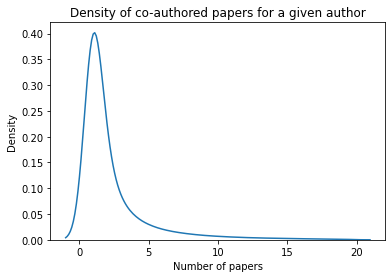
\includegraphics[width=1\linewidth]{3_chapter3/figures/density_author.png}
  \caption{}
  \label{fig:sub1}
\end{subfigure}%
\begin{subfigure}{.5\textwidth}
  \centering
  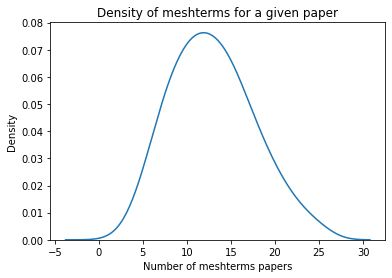
\includegraphics[width=1\linewidth]{3_chapter3/figures/density_meshterms.png}
  \caption{}
  \label{fig:sub2}
\end{subfigure}
\begin{subfigure}{.5\textwidth}
  \centering
  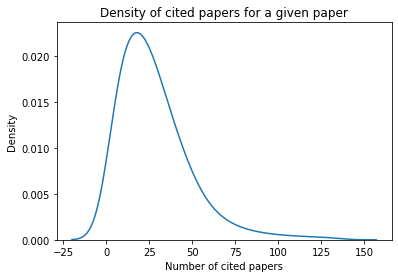
\includegraphics[width=1\linewidth]{3_chapter3/figures/density_cited_paper.png}
  \caption{}
  \label{fig:sub3}
\end{subfigure}
\caption[Density of number of authors, meshterms and references]{\justifying (a) Density of contribution of authors. On average an author has 2.6 publications (solo or co-authored) in 10 years. \\ (b) Density of the number of mesh terms between 2000-2010. On average, a paper is labelled with 13 mesh terms. \\(c) Density of references between 2000-2010. On average, a paper has 23 references }
\label{fig:10}
\end{figure}

\begin{figure}[H]
  \centering
  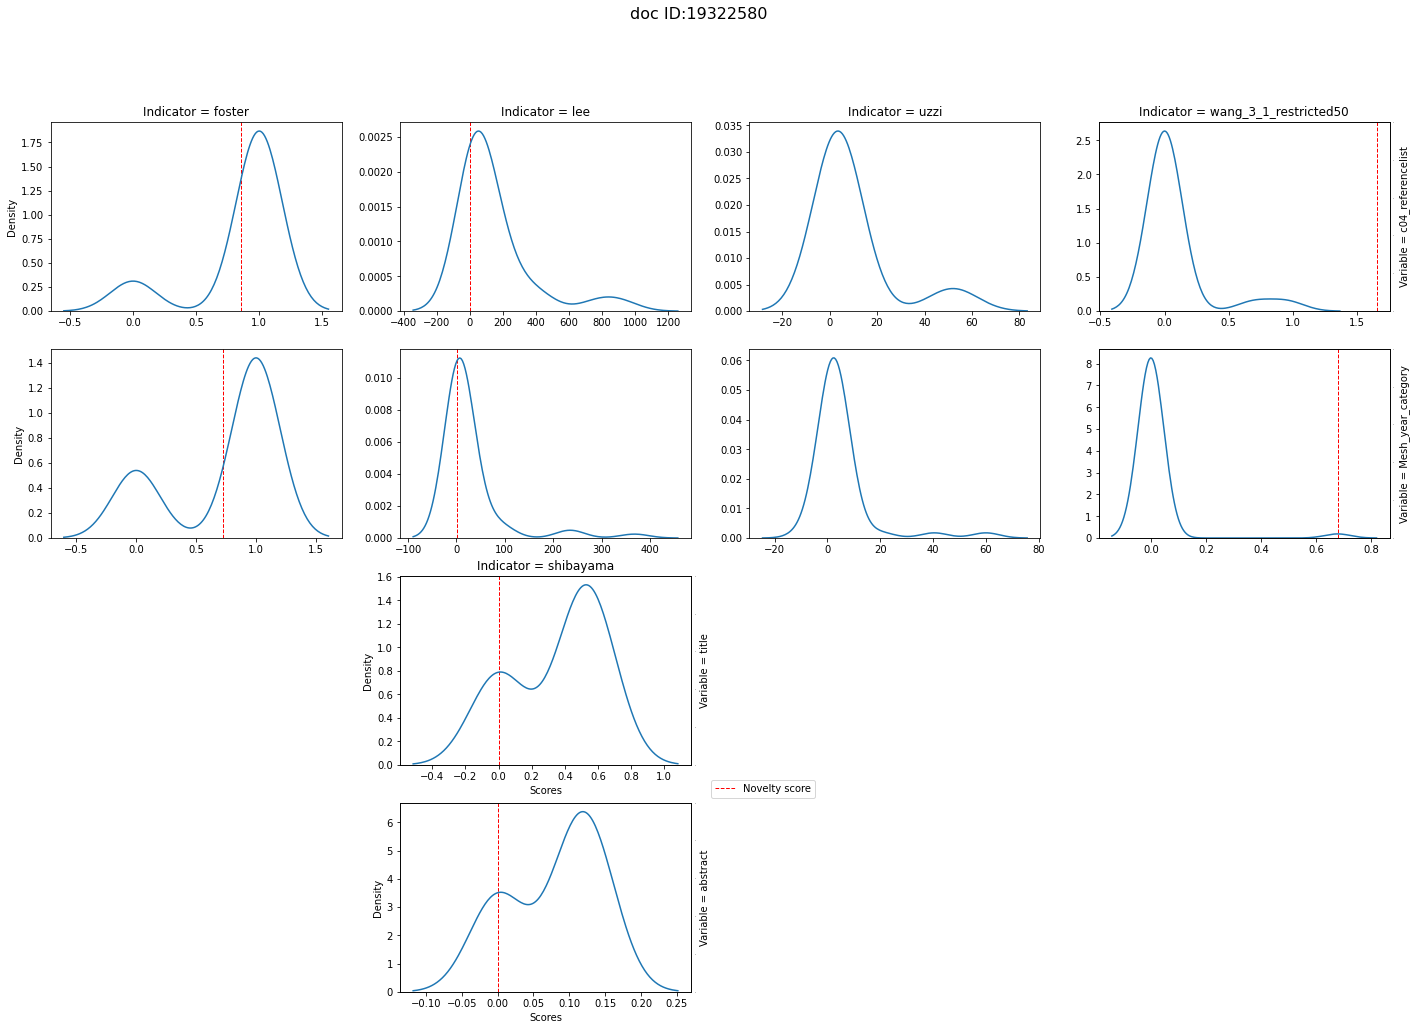
\includegraphics[scale=0.32]{3_chapter3/figures/density_score.png}
\caption[Distribution of novelty indicators for PMID 10698680]{\justifying Each combination has a novelty score. A single plot represents the density of score combinations for a specific paper (PMID 10698680) for a specific indicator and entity (i.e. mesh terms, journals, title, abstract). The scores for the first row were computed using a combination of cited journals. The scores for the second row were computed on mesh terms combinations. Each column represents an indicator. The last two rows are for text embedding-based indicators (i.e. \cite{shibayama2021measuring}: Novelty, Author proximity) on the title of the paper or abstract.}
\label{fig:11}
\end{figure}

\begin{figure}[H]
  \centering
  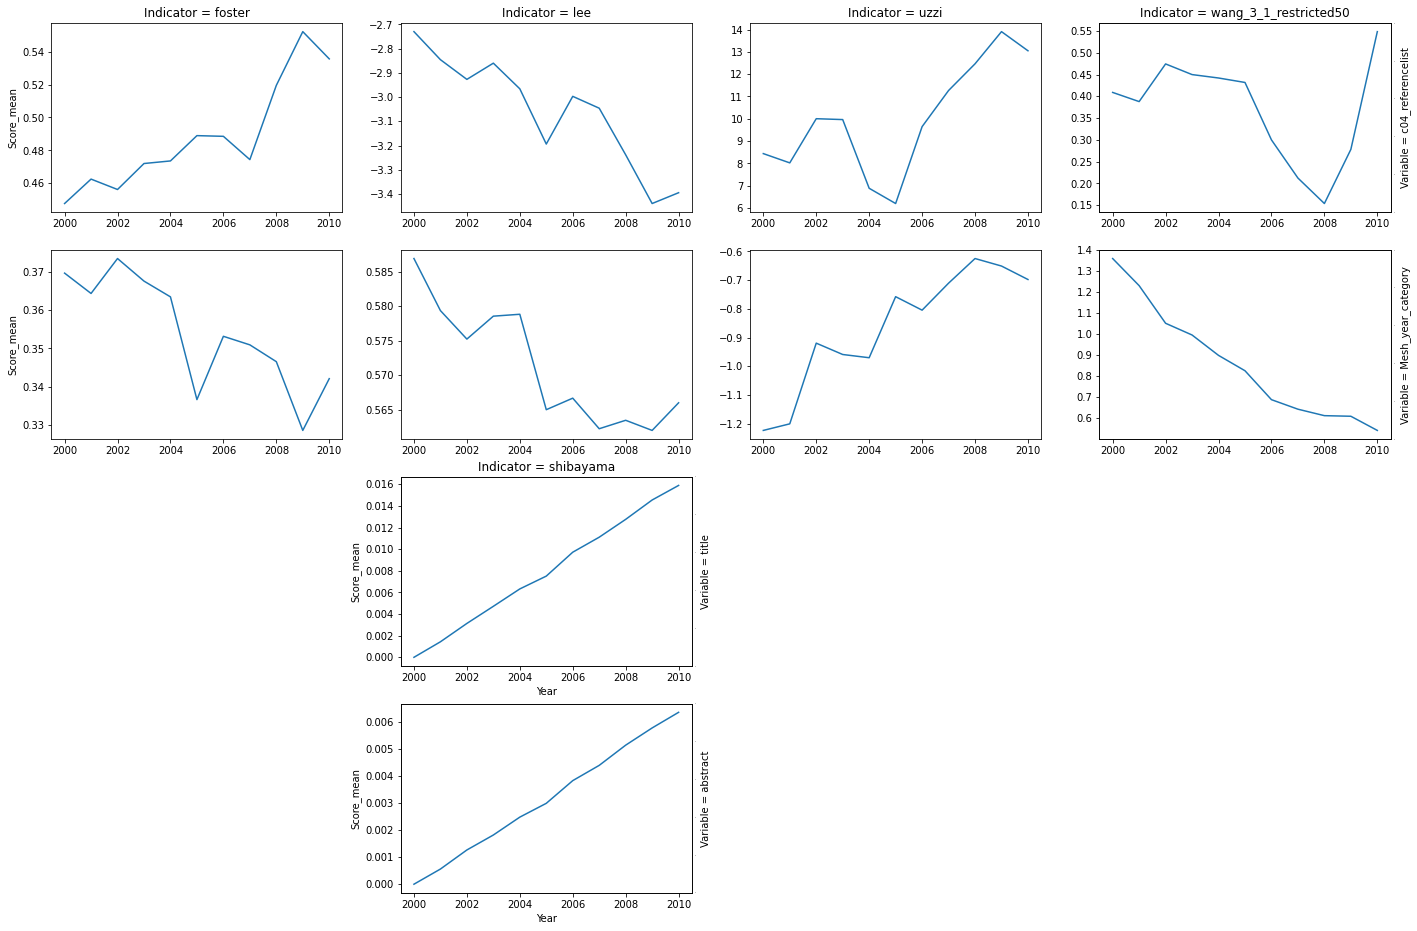
\includegraphics[scale=0.32]{3_chapter3/figures/trend_complex.png}
\caption[Novelty evolution over time]{\justifying The mean novelty score on every document for a given year. Columns and rows represent respectively indicators and variables.}
\label{fig:12}
\end{figure}

\begin{figure}[H]
  \centering
  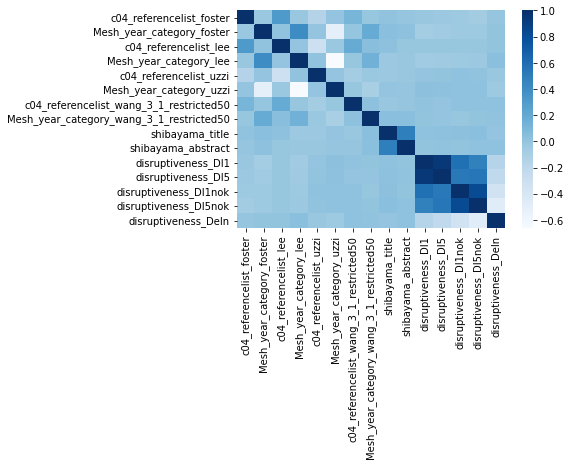
\includegraphics[width=0.63\linewidth]{3_chapter3/figures/heatmap.png}
\caption[Novelty indicators correlation]{\justifying The correlation between the novelty score for each indicator, given the entity, for the period 2000-2010}
\label{fig:13}
\end{figure}
